% !TeX root = ../../master.tex

\section{Nutzerhandbuch} % Nutzerhandbuch?
\label{sec:Nutzerhandbuch}

\subsection{Allgemein}

Das folgende Nutzerhandbuch wurde auf die drei vorgestellten Personas gemünzt, welche jeweils verschiedene Use-Cases der Anwendung darstellen sollen.
Dabei sind die Personas als Repräsentanten für echte Benutzer geplant.

So soll \duzi den Dozent darstellen, der gleichzeitig auch Administrator des Tools ist.
Dieser Dozent meldet sich dabei zunächst in der Anwendung, wie in \myRefGeneral{ssec:Einloggen} beschrieben, an.
Anschließend stehen ihm verschiendene Möglichkeiten zum weiteren Vorgehen zur Verfügung.
So kann er zunächst seine eigens erstellten und veröffentlichten Umfragen einsehen und sich die dazugehörigen Ergebnisse betrachten, wie es in \myRefGeneral{ssec:ResultDashboard} beschrieben wird.
Außerdem kann er über das \emph{Survey Master Paradise}, beschrieben in \myRefGeneral{ssec:SurveyMasterParadise}, seine Umfrage-Vorlagen verwalten und neue Vorlagen erstellen.
Das Erstellen neuer Vorlagen wird in \myRefGeneral{ssec:CreateMaster} näher beschrieben.

Als Administrator besitzt \duzi ebenfalls besondere Rechte, so kann er den Registrierungsschlüssel, näheres dazu in Kapitel \myRefGeneral{ssec:AdministratorTools}, anzeigen oder ändern.
Ebenfalls kann er einen neuen Nutzer anlegen, sofern Personen, die den Registrierungsschlüssel nicht erhalten dürfen, einen Account erhalten sollen, wie es etwa bei der Persona \ariane der Fall ist. 
Zudem kann ein Administrator alle im System vorhandene Personen einsehen, das Passwort dieser zurücksetzen oder diese zum Admin ernennen.

Als zweite Persona wurde die Studentin \ariane vorgestellt.
Diese möchte neben der Beantwortung von Umfragen, wie in \myRefGeneral{ssec:TeilnahmeAnEinerUmfrage} erläutert, auch selbst Umfragen erstellen, was näher in \myRefGeneral{ssec:CreateMaster} beschrieben wird.
Aufgrund von Personas wie \ariane ist es notwendig die SurveyMaster nur für den jeweiligen Ersteller sichtbar zu machen, sodass \textit{externe} Nutzer kein Zugriff auf potentiell geschützte Umfrage-Templates erhalten können.

Zu guter Letzt stellt die dritte Persona, \weigert, den Standardstudenten dar, der lediglich an einer Umfrage teilnehmen möchte und somit nur die Schritte, welche in Kapitel \myRefGeneral{ssec:TeilnahmeAnEinerUmfrage} beschrieben werden, befolgen muss.
Dabei ist der benötigte Aufwand so gering wie möglich, dass der Student die Umfrage schnell findet und einfach beantworten kann.
Zudem wird der Schutz der Daten des Teilnehmers einer solchen Umfrage besonders in den Vordergrund gerückt, da ein Rückschluss auf den Teilnehmer nur bei Umfragen, welche einer begrenzten Teilnehmerzahl zur Verfügung standen, grob möglich ist.

Die meisten Funktionen, welche eine Änderung des Datenzustands zur Folge haben, besitzen zudem eine zum Anwendungsfall passende Benachrichtigung.
Ein paar Beispiele dazu wurden in Kapitel \myRefGeneral{ssec:Meldungen} aufgezeigt.
Diese decken alle vorhandenen Meldungstypen ab, die Inhalte können jedoch abweichen.

\subsection{Einloggen}
\label{ssec:Einloggen}

In jedem Use-Case der Anwendung beginnt mit der in Abbildung \myRefGeneral{fig:EingabemaskeSurveycode} dargestellten Startansicht.
Um sich nun anzumelden muss zunächst der mit \desTwo markierte Knopf gedrückt werden, um zur in Abbildung \myRefGeneral{fig:Einloggen} dargestellten Seite, dem Login, zu kommen.
Anschließend muss der Nutzer sein vorher in \myRefGeneral{ssec:NutzerAnlegen} festgelegten Nutzernamen sowie Passwort in die jeweiligen Felder (\desOne, \desTwo) eintragen und über den \emph{Login}-Knopf anmelden.
Danach erfolgt eine automatische Weiterleitung zur in \myRefGeneral{ssec:ResultDashboard} abgebildeten Übersicht der offenen Umfragen.

\begin{figure}[H]
	\centering
	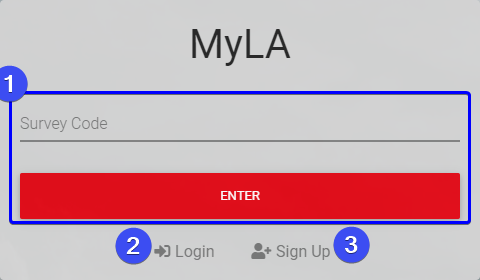
\includegraphics[width=0.5\textwidth, keepaspectratio]{img/guide/SurveyCode.png}
	\captionsetup{justification=centering, format=plain}
	\caption[Eingabemaske Surveycode]{Eingabemaske des Surveycodes \\\quelleScreenshot}
	\label{fig:EingabemaskeSurveycode}
\end{figure}

\begin{figure}[H]
	\centering
	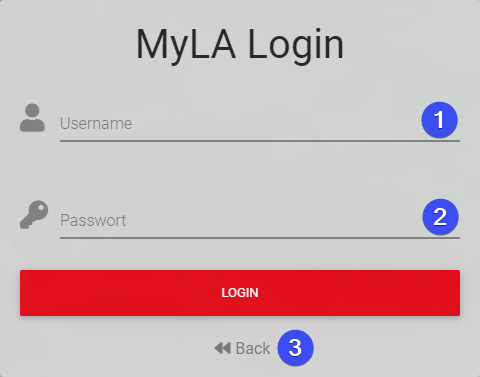
\includegraphics[width=0.5\textwidth, keepaspectratio]{img/guide/Login.png}
	\captionsetup{justification=centering, format=plain}
	\caption[Eingabemaske Einloggen]{Eingabemaske Einloggen \\\quelleScreenshot}
	\label{fig:Einloggen}
\end{figure} 

\subsection{Nutzer anlegen}
\label{ssec:NutzerAnlegen}

Ein Nutzer kann über zwei Arten angelegt werden.
Einerseits ist es einer Person, die den Registrierungsschlüssel kennt, möglich sich selbst zu Registrieren, wie es in Abbildung \myRefGeneral{fig:Register} gekennzeichnet wird.
Dabei muss der Nutzer in \desOne seinen gewünschten Nutzernamen eingeben, in \desTwo den festgelegten Registrierungsschlüssel und anschließend in \desThree und \desFour das gewünschte Passwort.
Falls der Registrierungsvorgang abgebrochen werden soll, kann der durch \desFive markierte Zurück-Knopf verwendet werden, welcher den Nutzer zurück auf die Startseite leitet.
Andererseits kann ein Administrator einen Nutzer anlegen, was jedoch genauer im Kapitel \myRefGeneral{ssec:AdministratorTools} beschrieben wird.

\begin{figure}[H]
	\centering
	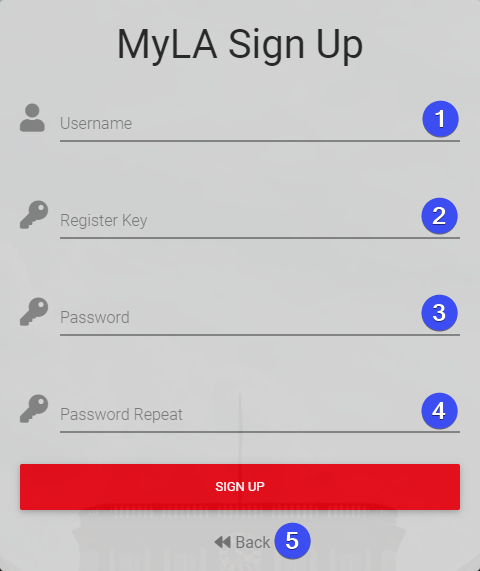
\includegraphics[width=0.5\textwidth, keepaspectratio]{img/guide/Register.png}
	\captionsetup{justification=centering, format=plain}
	\caption[Eingabemaske Registrierung]{Eingabemaske des Surveycodes \\\quelleScreenshot}
	\label{fig:Register}
\end{figure}

\subsection{Passwort ändern}

Jeder Nutzer ist in der Lage sein Passwort zu ändern, dies kann er über sein Profil, zu finden über der Navigationsleiste, die in Kapitel \myRefGeneral{ssec:NavBar} beschrieben wird, erledigen.
Dabei muss der Nutzer zunächst, wie in \myRefGeneral{fig:ChangeOwnPassword} dargestellt, sein altes Passwort in \desOne angeben und in \desTwo sowie \desThree sein neues einfügen und wiederholen.
Sofern ein Nutzer sein Passwort vergisst, kann ein Administrator dieses zurücksetzen.
Dazu wählt er im Administrationsbereich \myRefGeneral{ssec:AdministratorTools} den jeweiligen Nutzer aus und setzt dessen Password über das in Abbildung \myRefGeneral{fig:ChangePasswordOfUser} gezeigte Popup neu.
Sofern der Nutzer sich nun mit dem neu festgelegten Passwort anmeldet, wird dieser zur eigenständigen Aktualisierung des Passworts über die vorher beschriebene Art gezwungen.

\begin{figure}[H]
	\centering
	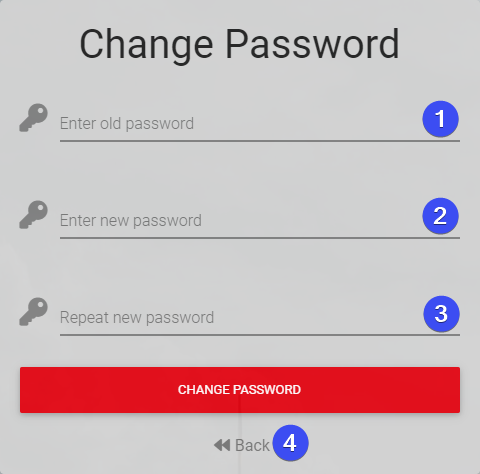
\includegraphics[width=0.5\textwidth, keepaspectratio]{img/guide/ChangeOwnPassword.png}
	\captionsetup{justification=centering, format=plain}
	\caption[Eingabemaske eigenes Passwort ändern]{Eingabemaske eigenes Passwort ändern \\\quelleScreenshot}
	\label{fig:ChangeOwnPassword}
\end{figure}

\begin{figure}[H]
	\centering
	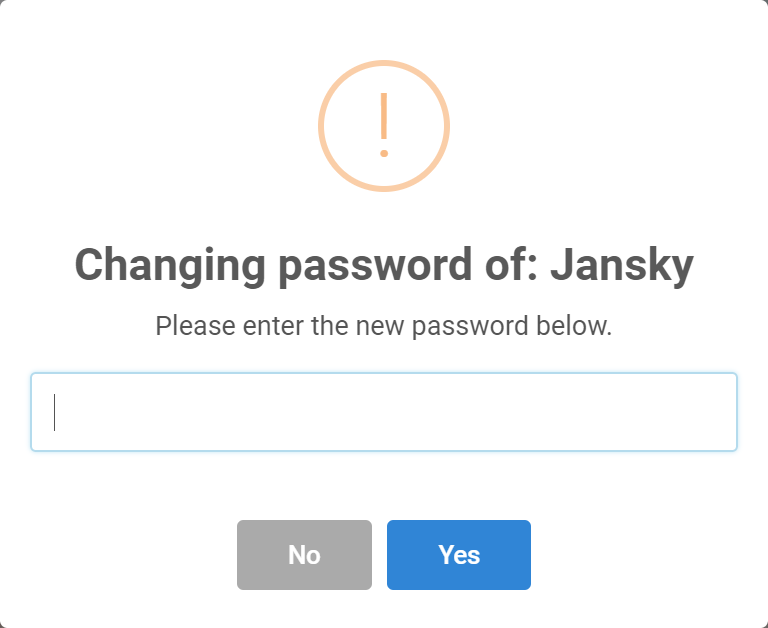
\includegraphics[width=0.5\textwidth, keepaspectratio]{img/guide/ChangePassword.png}
	\captionsetup{justification=centering, format=plain}
	\caption[Eingabemaske Passwort zurücksetzen]{Eingabemaske Passwort zurücksetzen \\\quelleScreenshot}
	\label{fig:ChangePasswordOfUser}
\end{figure}

\subsection{Result Dashboard}
\label{ssec:ResultDashboard}

Sobald ein Nutzer sich anmeldet landet er auf der Übersicht der aktiven Umfragen, dargestellt in Abbildung \myRefGeneral{fig:ResultDashboard}.
Hier sieht der Nutzer zunächst, wie auf jeder weiteren Hauptseite, den aktuellen Seitennamen, welcher in der Abbildung durch \desOne markiert wird.
\desTwo markiert eine Suchleiste, in der bestimmte Umfragen aus allen dargestellten Umfragen herausgefiltert werden können, sodass auch Nutzer, die bereits eine große Anzahl an Umfragen erstellt haben, alle schnell finden können.
Umfragen sind auf dieser Ansicht allgemein als Karten aufgebaut, wie \desThree zeigt.
Dabei besitzen diese einen eigenen Titel sowie den Titel der Vorlage und die Beschreibung dieser.
Zudem wird die Teilnehmeranzahl der aktiven Umfrage angezeigt, sodass der aktuelle Stand der Umfrage beobachtet werden kann, ohne die Ergebnisse auswerten zu müssen.
Des Weiteren wird der Surveycode besonders hervorgehoben, um auch zu vorbereiteten Umfragen die Codes griffbereit zu haben.
\faClipboard\xspace ermöglicht es zudem den Direktlink zur Umfrage automatisch in die Zwischenablage zu kopieren, um diesen an die potentiellen Teilnehmer weiterleiten zu können.

\begin{figure}[H]
	\centering
	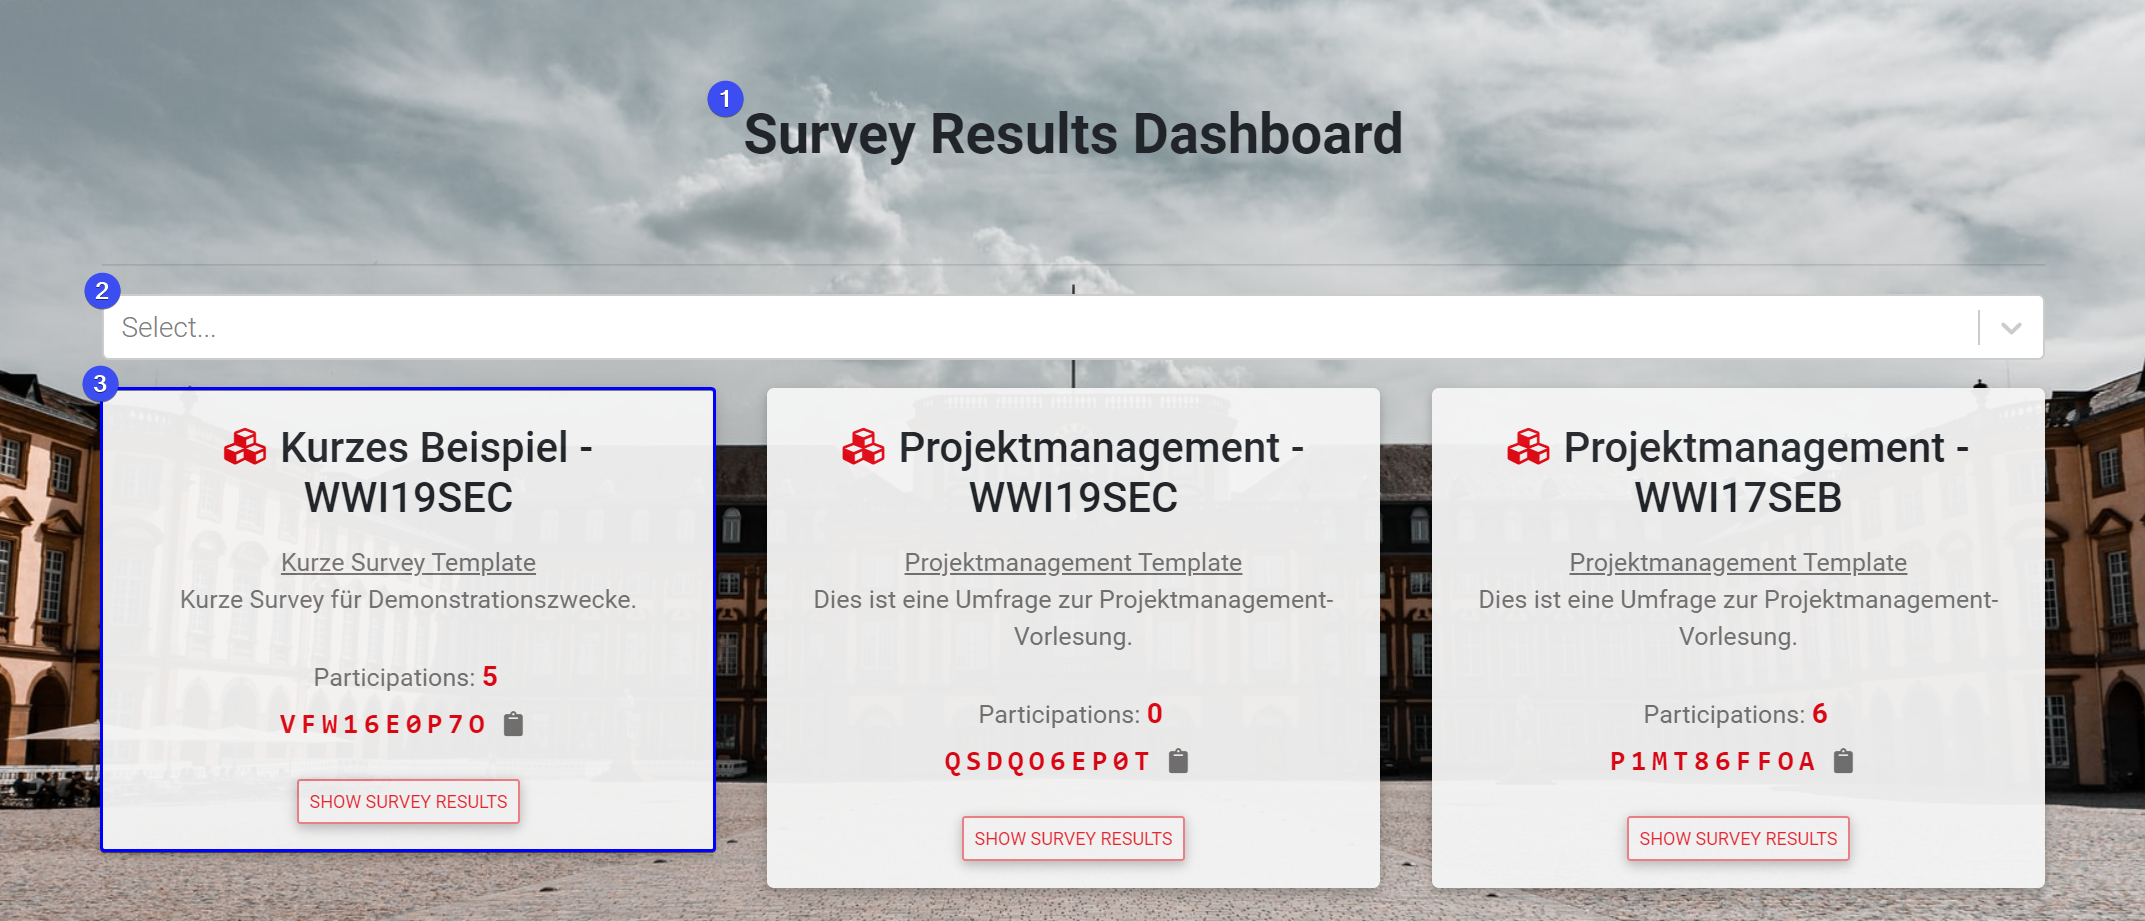
\includegraphics[width=0.5\textwidth, keepaspectratio]{img/guide/ResultDashboard.png}
	\captionsetup{justification=centering, format=plain}
	\caption[Übersicht aktive Umfragen]{Übersicht aktive Umfragen \\\quelleScreenshot}
	\label{fig:ResultDashboard}
\end{figure}


\subsection{Teilnahme an einer Umfrage}
\label{ssec:TeilnahmeAnEinerUmfrage}

Um an einer Umfrage teilzunehmen, muss der Partizipant, wie in Schritt \desOne in \abb \myRefGeneral{fig:EingabemaskeSurveycode} dargestellt, einen \emph{Surveycode} eingeben.
Da das Partizipieren ein Kernpunkt der Anwendung darstellt, ist dies als Startseite.
Der Benutzer bzw. Teilnehmer hat zudem die Möglichkeit über den Button \enquote{Login} \desTwo auf die Login-Seite zu navigieren (Kap. \vref{ssec:Login}). 
Oder alternativ über den Button \enquote{Sign Up} \desThree, die Registrierungsseite (Kap. \vref{ssec:NutzerAnlegen}) aufrufen.

% \desFour, \desFive, \desSix, \desSeven, \desEight, \desNine

\begin{figure}[H]
	\centering
	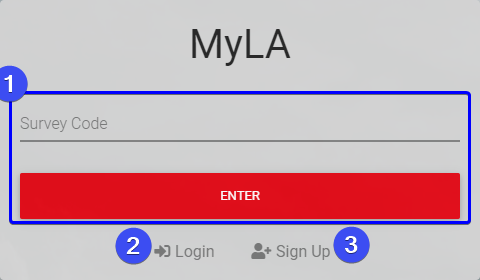
\includegraphics[width=0.5\textwidth, keepaspectratio]{img/guide/SurveyCode.png}
	\captionsetup{justification=centering, format=plain}
	\caption[Eingabemaske Surveycode]{Eingabemaske des Surveycodes \\\quelleScreenshot}
	\label{fig:EingabemaskeSurveycode}
\end{figure}

\abb \myRefGeneral{fig:Teilnehmermaske} stellt die Teilnehmermaske der Umfrage durch. 
\desOne zeigt den Titel der Umfrage (hier: Projektmanagement -- WWI17SEB). 
\desTwo zeigt die Beschreibung der Umfrage (hier: Dies ist eine Umfrage zur Projektmanagement-Vorlesung). 
\desThree ist das Hauptelement der Seite.
Sie zeigt die eigentliche Umfrage.
Über den Button \enquote{Complete} kann der Teilnehmer die Umfrage abschließen. 
Er erhält ein visuelles Feedback. 

\begin{figure}[H]
	\centering
	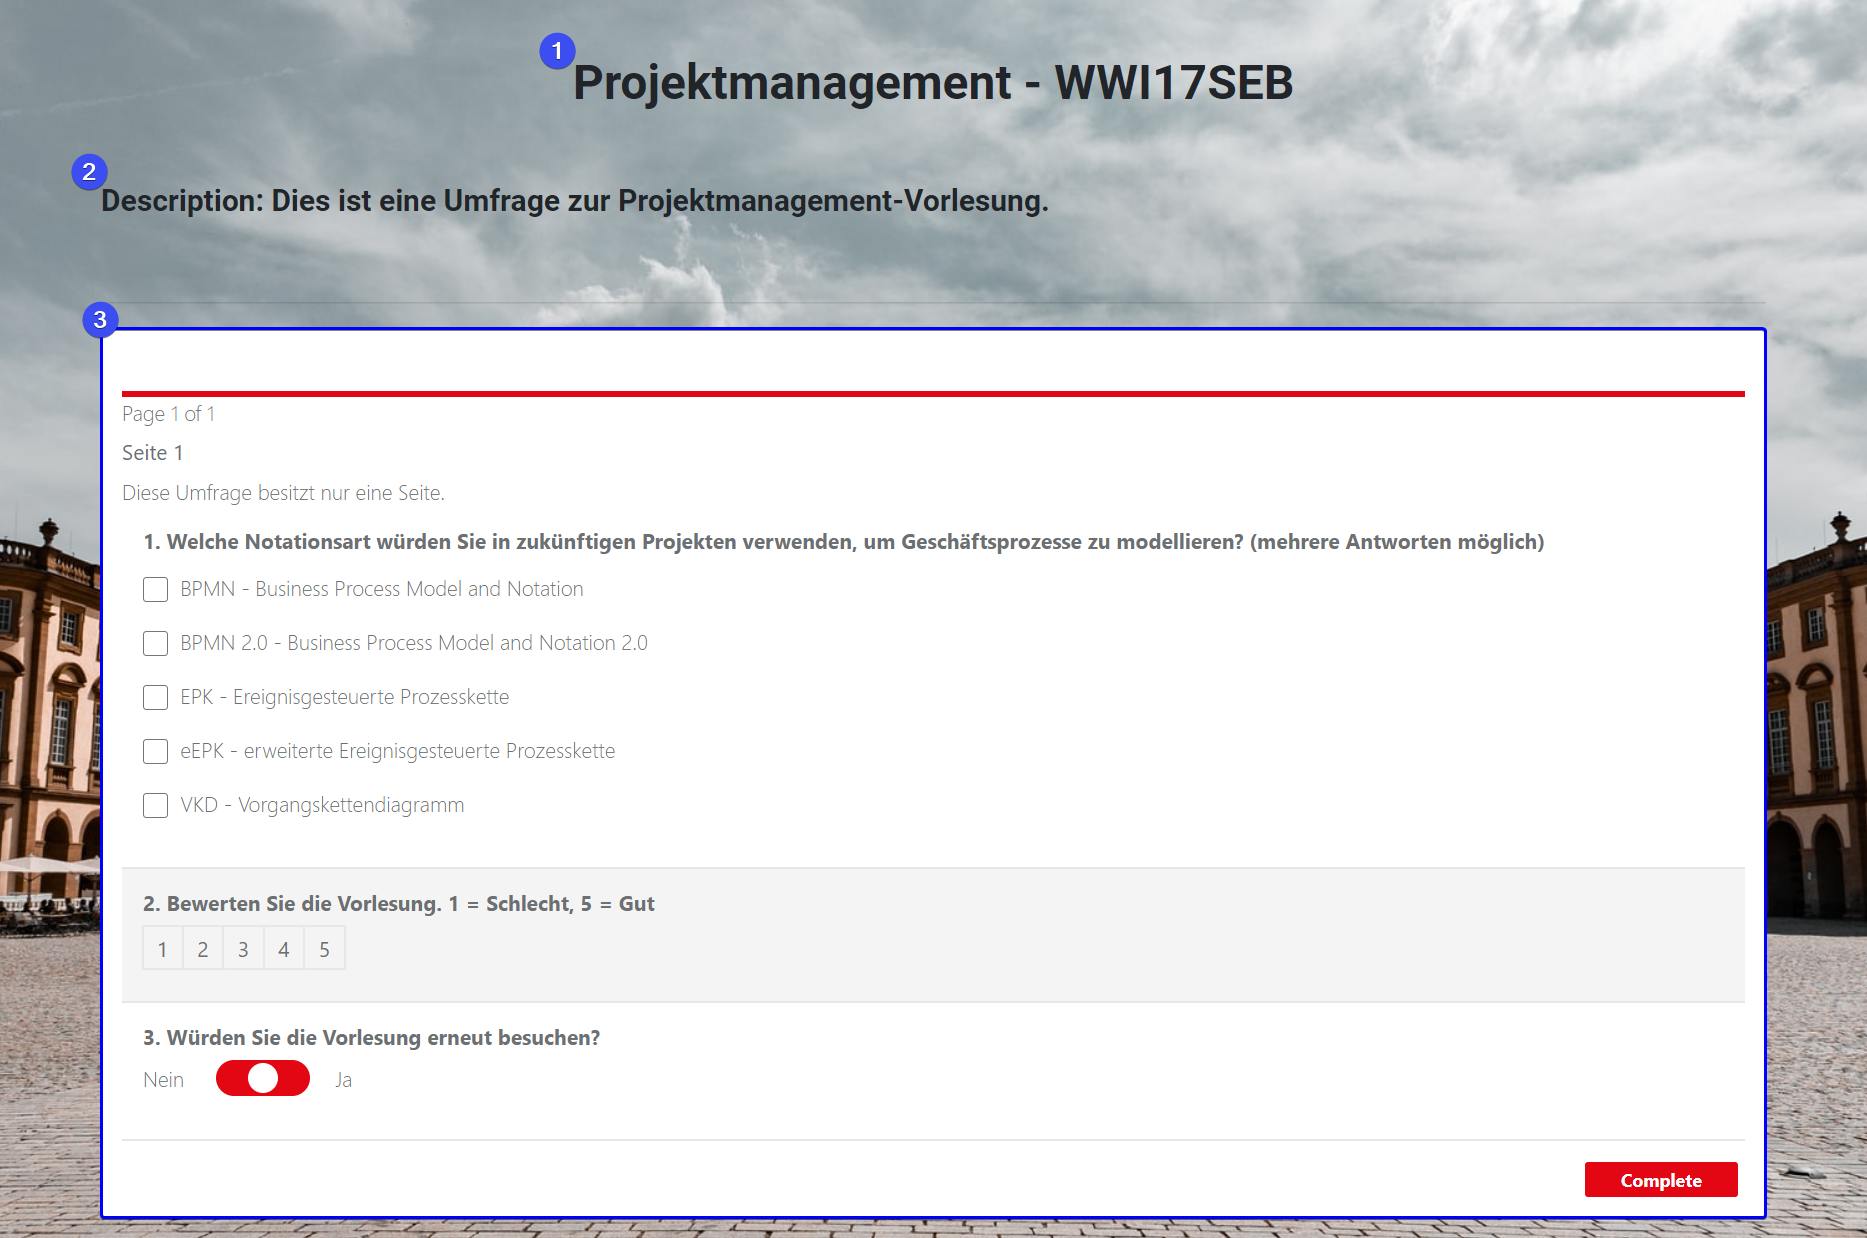
\includegraphics[width=0.70\textwidth, keepaspectratio]{img/guide/SurveyParticipate.png}
	\captionsetup{justification=centering, format=plain}
	\caption[Teilnehmermaske]{Teilnehmermaske \\\quelleScreenshot}
	\label{fig:Teilnehmermaske}
\end{figure}

\subsection{Erstellen einer Umfrage}
\label{ssec:CreateMaster}

Das Kernelement dieser Anwenndung ist das Erstellen von Umfragen. 
\abb \myRefGeneral{fig:Umfrageeditor} zeigt den Editor zum Erstellen oder Bearbeiten einer Umfrage. \newline
Der Benutzer kann hier einen Titel und Beschreibung für seine Umfrage wählen. 
Über den in der linken Seite befindlichen Navigationsbereich kann der Benutzer verschiedene Elemente wie \ua: 
% 
\begin{itemize}
    \item Single-/Multiple Choice
    \item Ja/Nein Antworten
    \item Freitextfelder
    \item Bewertungsskala (Skala frei wählbar)
    \item Singleinput
    \item Auswahl von Bildern
\end{itemize}
% 

Im oberen Bereich des Editors befindet sich die Pagination. 
Der Benutzer kann hier seine Umfrage strukturieren, indem er eine neue Seite der Umfrage hinzufügt. 
Darüber hinaus kann er stets zwischen den Seiten auswählen. 

Den im rechten Teil befindlichen Navigationsbereich beinhaltet die \ua die Menüsprache (hier: englisch). 
Darüber hinaus können Zeitintervalle festgelegt werden, indem die Umfrage zu bewerten ist (Timer). 

Über den Button \enquote{Save Survey} kann der Benutzer seine Umfrage speichern. 
Er erhält ein visuelles Feedback. 

\begin{figure}[H]
	\centering
	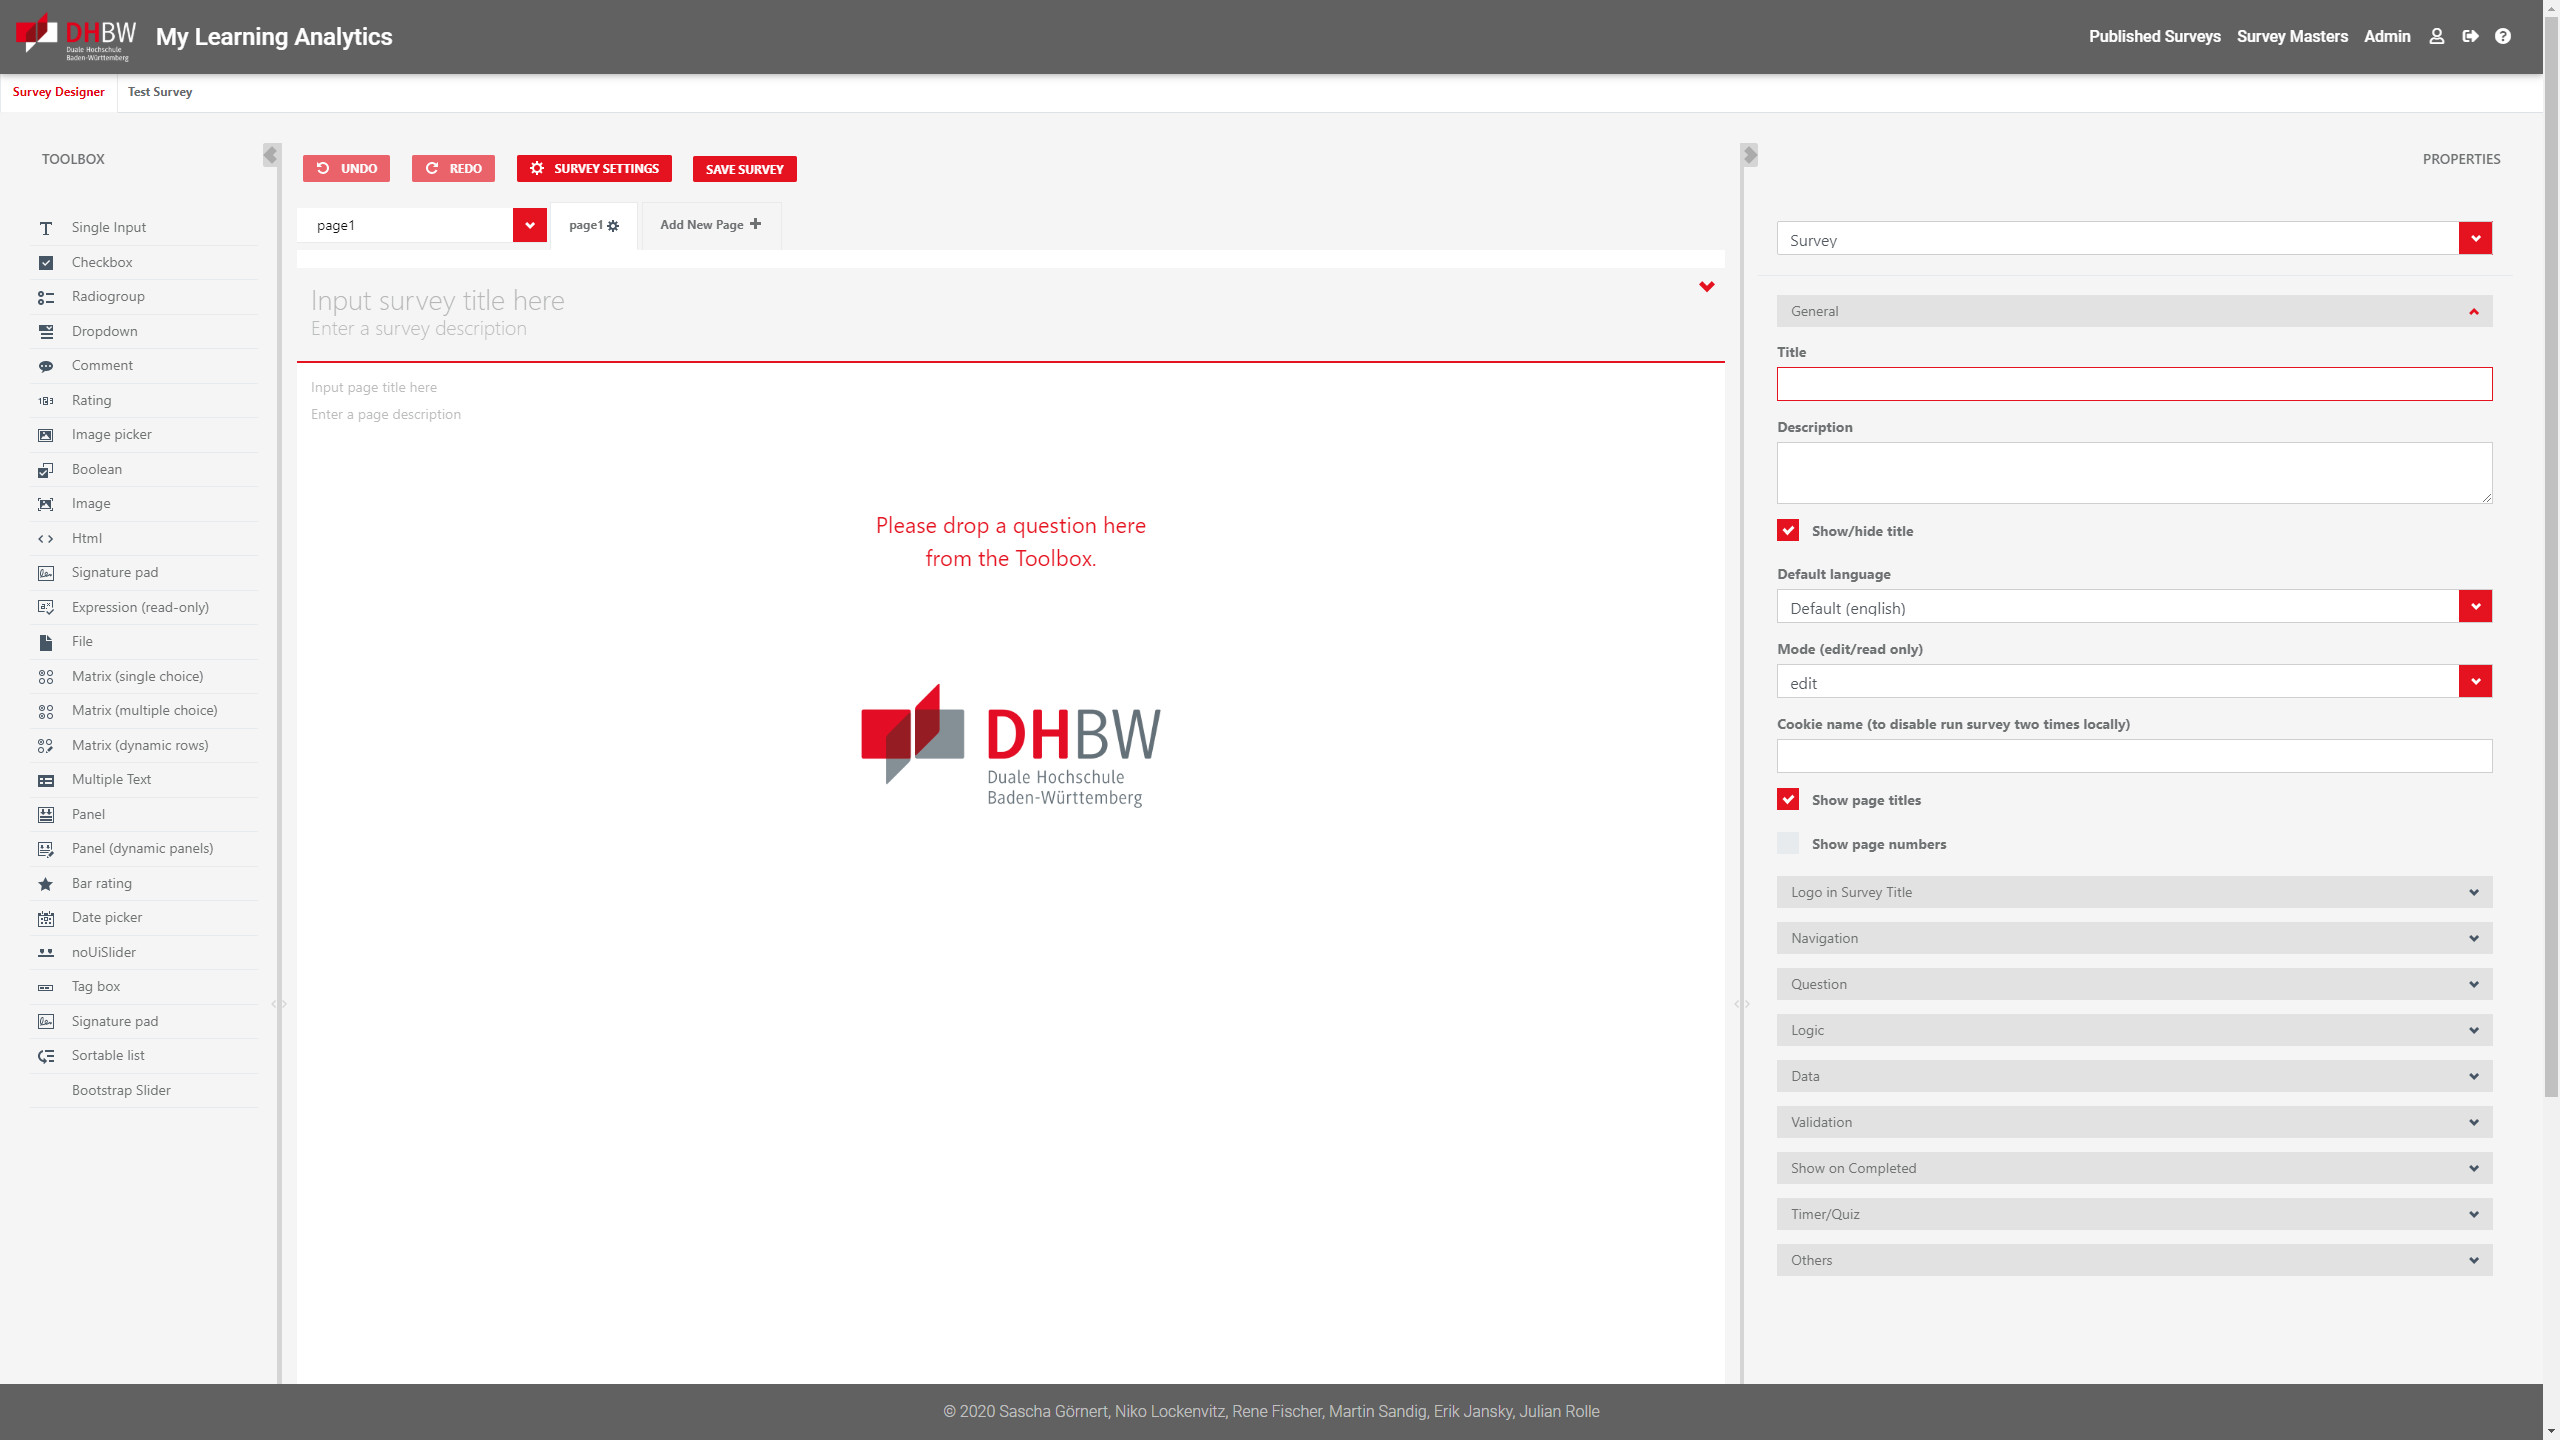
\includegraphics[width=0.95\textwidth, keepaspectratio]{img/guide/SurveyTemplate.png}
	\captionsetup{justification=centering, format=plain}
	\caption[Umfrageeditor]{Umfrageeditor \\\quelleScreenshot}
	\label{fig:Umfrageeditor}
\end{figure}

\subsection{Administrator Tools}
\label{ssec:AdministratorTools}

\abb \vref{fig:AdminSpace} zeigt den Administrationsbereich der Anwendung. 
Der Benutzer kann hier, wie in \desOne dargestellt, den Registrierungsschlüssel zum Registrieren eines neuen Benutzers einsehen oder neu vergeben (vgl. Abb. \vref{fig:EditRegisterKey} \& Abb. \vref{fig:NewRegisterkey}). \newline
\desTwo zeigt die Möglichkeit des Erstellens eines neuen Benutzers (vgl. Kap. \vref{fig:NeuenBenutzerAnlegen}). 
Über das in \desThree dargestellte Karte kann der Administrator alle Benutzer im System anzeigen (vgl. Kap. \vref{fig:UserSpace}).

\begin{figure}[H]
	\centering
	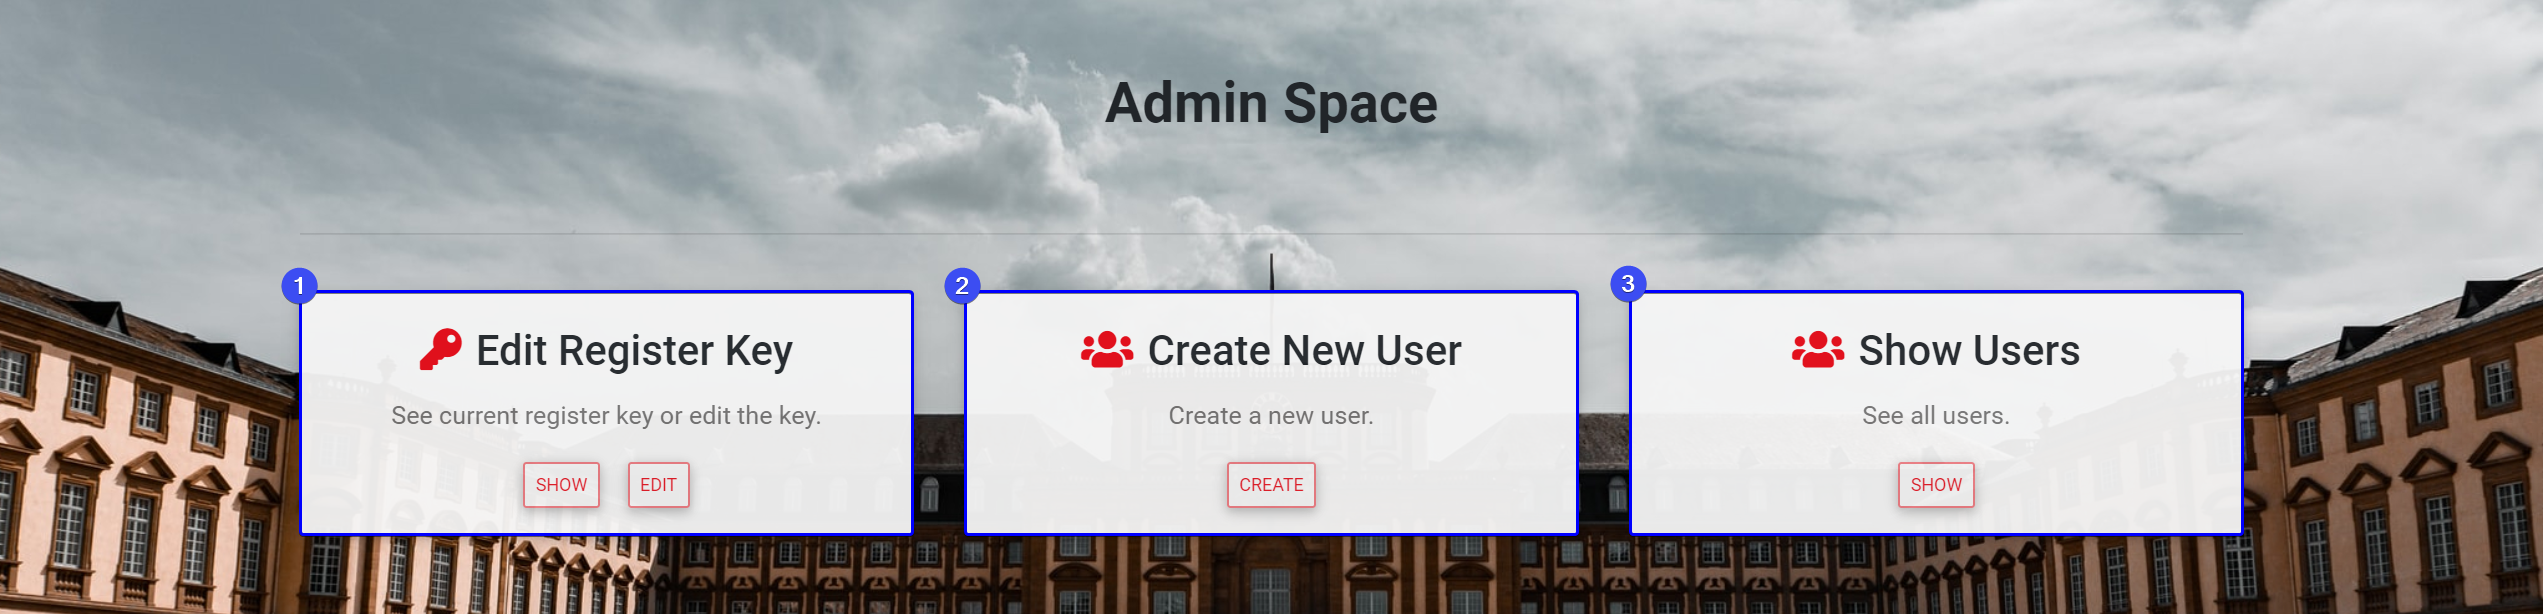
\includegraphics[width=0.70\textwidth, keepaspectratio]{img/guide/AdminSpace.png}
	\captionsetup{justification=centering, format=plain}
	\caption[Administrationsbereich]{Administrationsbereich \\\quelleScreenshot}
	\label{fig:AdminSpace}
\end{figure}

\begin{figure}[H]
	\centering
	
\includegraphics[width=0.5\textwidth, keepaspectratio]{img/guide/RegisterKey.png}
	\captionsetup{justification=centering, format=plain}
	\caption[Neuer Registrierungsschlüssel]{Neuer Registrierungsschlüssel \\\quelleScreenshot}
	\label{fig:NewRegisterkey}
\end{figure}

\begin{figure}[H]
	\centering
	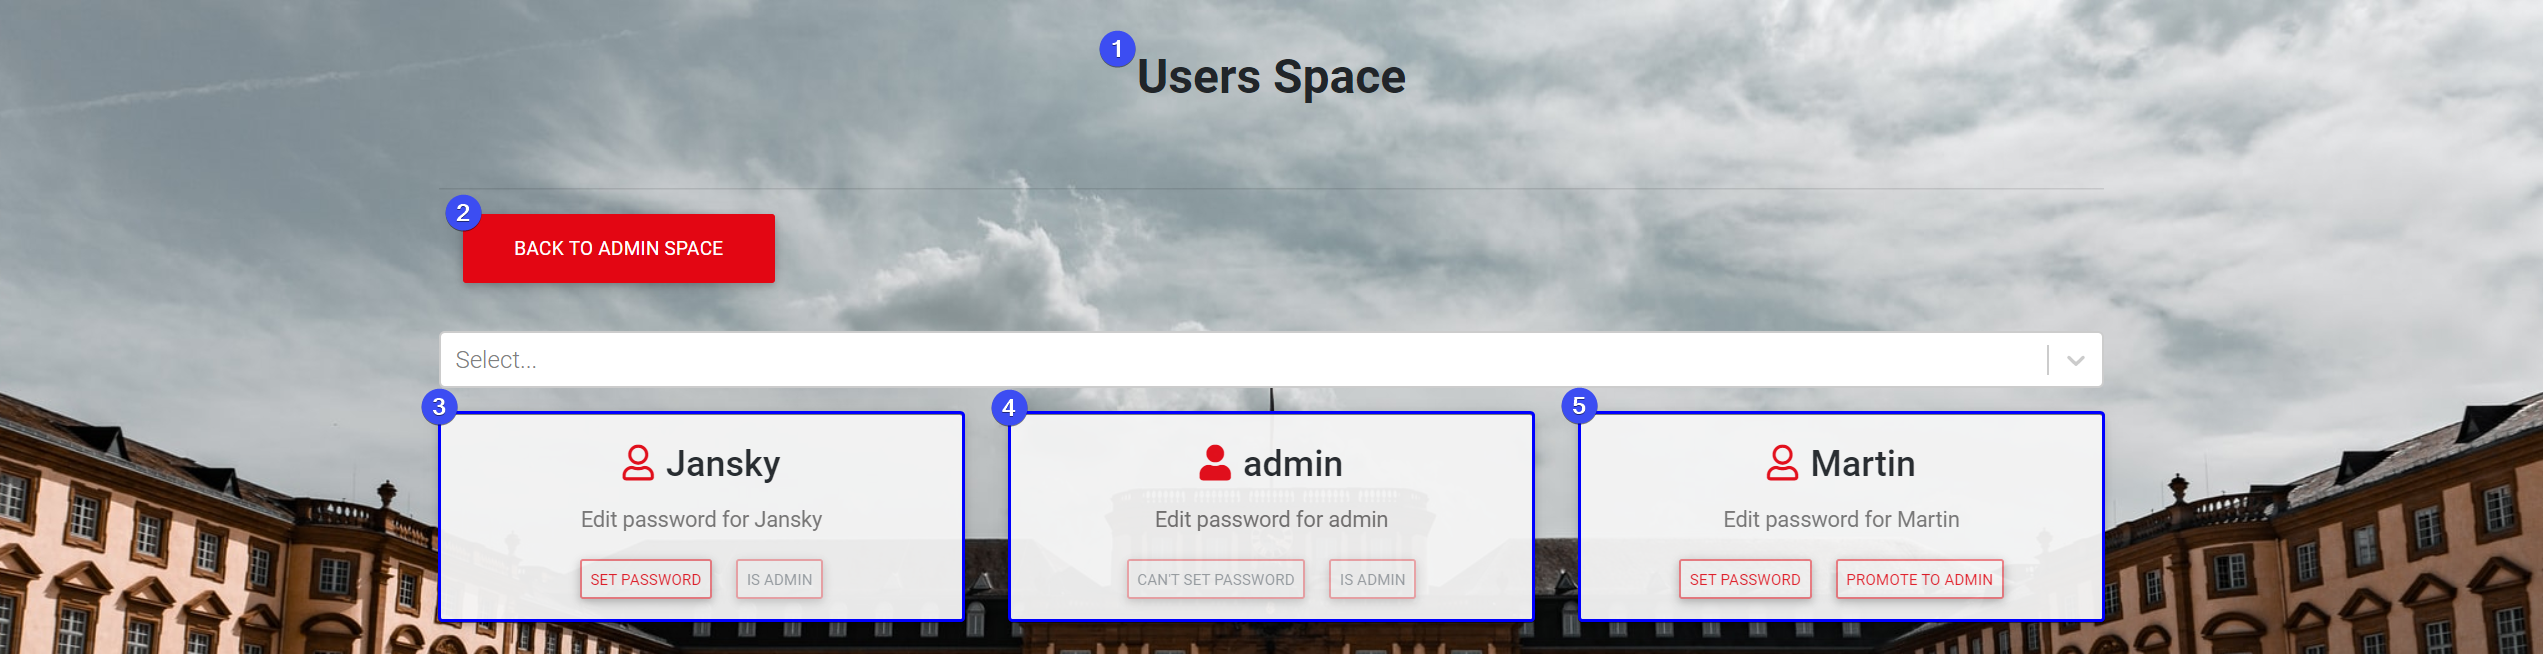
\includegraphics[width=0.5\textwidth, keepaspectratio]{img/guide/UserSpace.png}
	\captionsetup{justification=centering, format=plain}
	\caption[In der Anwendung befindliche Personen]{In der Anwendung befindliche Personen \\\quelleScreenshot}
	\label{fig:UserSpace}
\end{figure}

\begin{figure}[H]
	\centering
	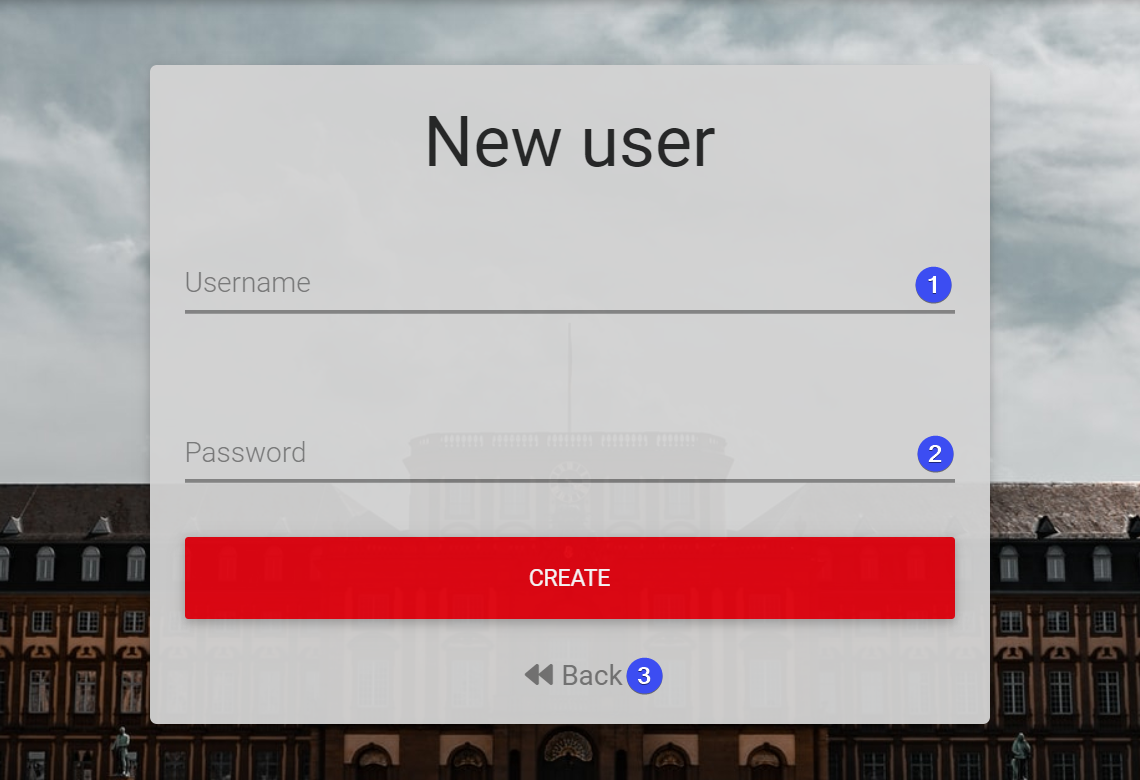
\includegraphics[width=0.5\textwidth, keepaspectratio]{img/guide/NewUser.png}
	\captionsetup{justification=centering, format=plain}
	\caption[Neuen Benutzer anlegen]{Neuen Benutzer anlegen \\\quelleScreenshot}
	\label{fig:NeuenBenutzerAnlegen}
\end{figure}


\begin{figure}[H]
	\centering
	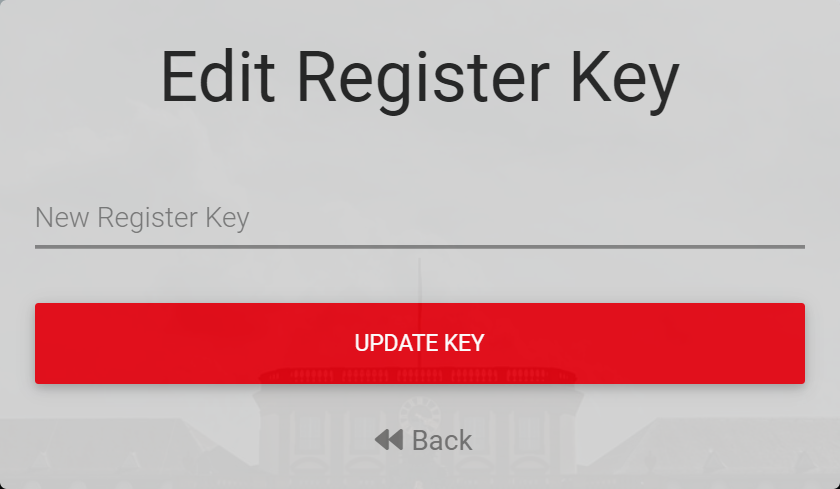
\includegraphics[width=0.5\textwidth, keepaspectratio]{img/guide/EditRegisterKey.png}
	\captionsetup{justification=centering, format=plain}
	\caption[Editieren des Registrierungsschlüssel]{Editieren des Registrierungsschlüssel \\\quelleScreenshot}
	\label{fig:EditRegisterKey}
\end{figure}



%%%%%%%%% --------------------- %%%%%%%%%%%%%%%
\subsection{Eigener Account}
\label{ssec:EigenerAccount}

Ziele es für die angemeldeten Benutzer wie \duzi oder die Studentin \ariane ihren Account verwalten können. 
\abb \myRefGeneral{fig:MyAccount} zeigt die Benutzeroberfläche. \newline
Hier können sie ihr Passwort ändern. 
\abb \myRefGeneral{fig:ChangeOwnPassword} zeigt die Passwortwechsel-Oberfläche. 
Um das Ändern des Passworts zu bestätigen, müssen diese wie in \desOne zu erst ihr altes Passwort eingeben. 
Anschließend wählen sie wie in \desTwo das neue Passwort und bestätigen dies in \desThree. 
Über den Button \enquote{Change Password} können die Protagonisten das Passwort wechseln. 
Alternativ können sie über den Zurück-Button \desFour wieder auf den Account navigieren. 
% 
\begin{figure}[H]
	\centering
	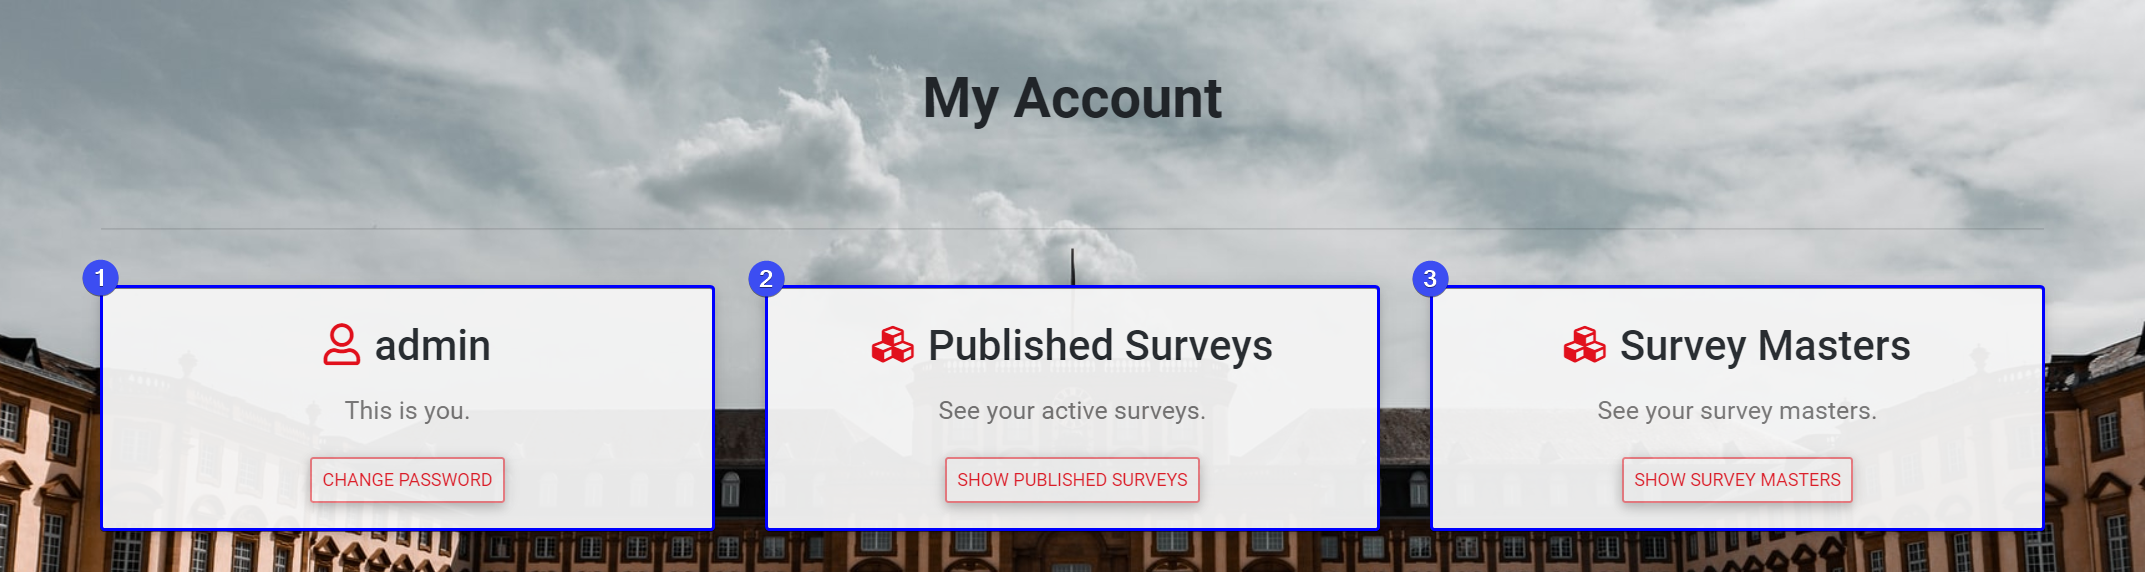
\includegraphics[width=0.5\textwidth, keepaspectratio]{img/guide/MyAccount.png}
	\captionsetup{justification=centering, format=plain}
	\caption[Account]{Account\\\quelleScreenshot}
	\label{fig:MyAccount}
\end{figure}
% 
\begin{figure}[H]
	\centering
	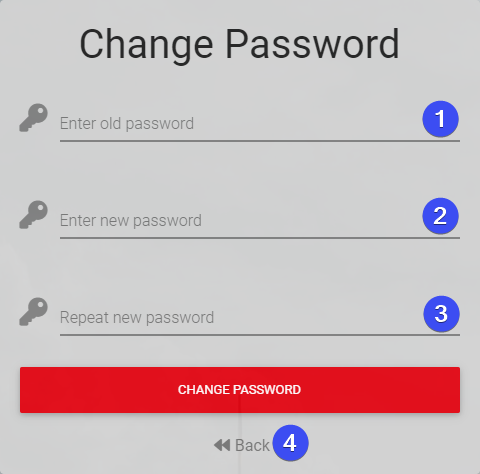
\includegraphics[width=0.5\textwidth, keepaspectratio]{img/guide/ChangeOwnPassword.png}
	\captionsetup{justification=centering, format=plain}
	\caption[Passwortändern (Benutzeransicht)]{Passwortändern (Benutzeransicht)\\\quelleScreenshot}
	\label{fig:ChangeOwnPassword}
\end{figure}
% 
%%%%%%%%% --------------------- %%%%%%%%%%%%%%%
\subsection{Survey Master Paradise}
\label{ssec:SurveyMasterParadise}
Survey Master Paradise ist einer der Hauptkomponenten dieser Anwendung. 
Hier können die Benutzer der Anwendung, wie \duzi und die Studentin \ariane, ihre erstellen Umfragen einsehen. 
\abb \vref{fig:SurveyMasterParadise} zeigt die Umfrage Seite. 
Hintergrund dieser Seite ist, dass \duzi verschiedene Umfragen erstellen kann, die er in seinen verschiedenen Kursen wie \zb \emph{WWWI17SEB} oder \emph{WWWI18SEA} zur Beantwortung heranziehen kann. % sorry kopf is mad: s
Da die Protagonisten, \duzi und die Studentin \ariane, durch ihren vielen Umfragen an einer renomierten Universität, im Laufe der Zeit viele Umfragen erstellt. 
\desTwo bietet den Benutzern die Möglichkeit ihre Vorlagen nach Umfragename wie \zb \emph{Projektmanagement Template} zu filtern. 
Über \desThree können die Benutzer eine neue Vorlage erstellen (vgl. Kap. \vref{ssec:CreateMaster}). \newline
Über die in \desFour können die Benutzer ihre Vorlagen unter einem bestimmten Titel für die Teilnehmer wie \weigert publiziert werden (Publish Survey). 
Die Anzahl der Publikation ist für die Protagonisten ersichtlicht (Times published). \newline
Die Icons wie in \desFive dargestellt, bieten dem Benutzer die Möglichkeit, sofern er noch keine Umfrage publiziert hat:
% 
\begin{itemize}
    \item seine Umfrage zu editieren \faEdit
    \item seine Umfrage zu kopieren \faCopy
    \item oder zu löschen \faTrash.
\end{itemize}
% 
Hat \zb \duzi mindestens eine Umfrage, basierend auf seiner Vorlage, publiziert, so stehen ihm noch die Funktionen:
\begin{itemize}
    \item Umfrage kopieren \faCopy
    \item und \faIdCard
\end{itemize} 

zur Verfügung. 

\begin{figure}[H]
	\centering
	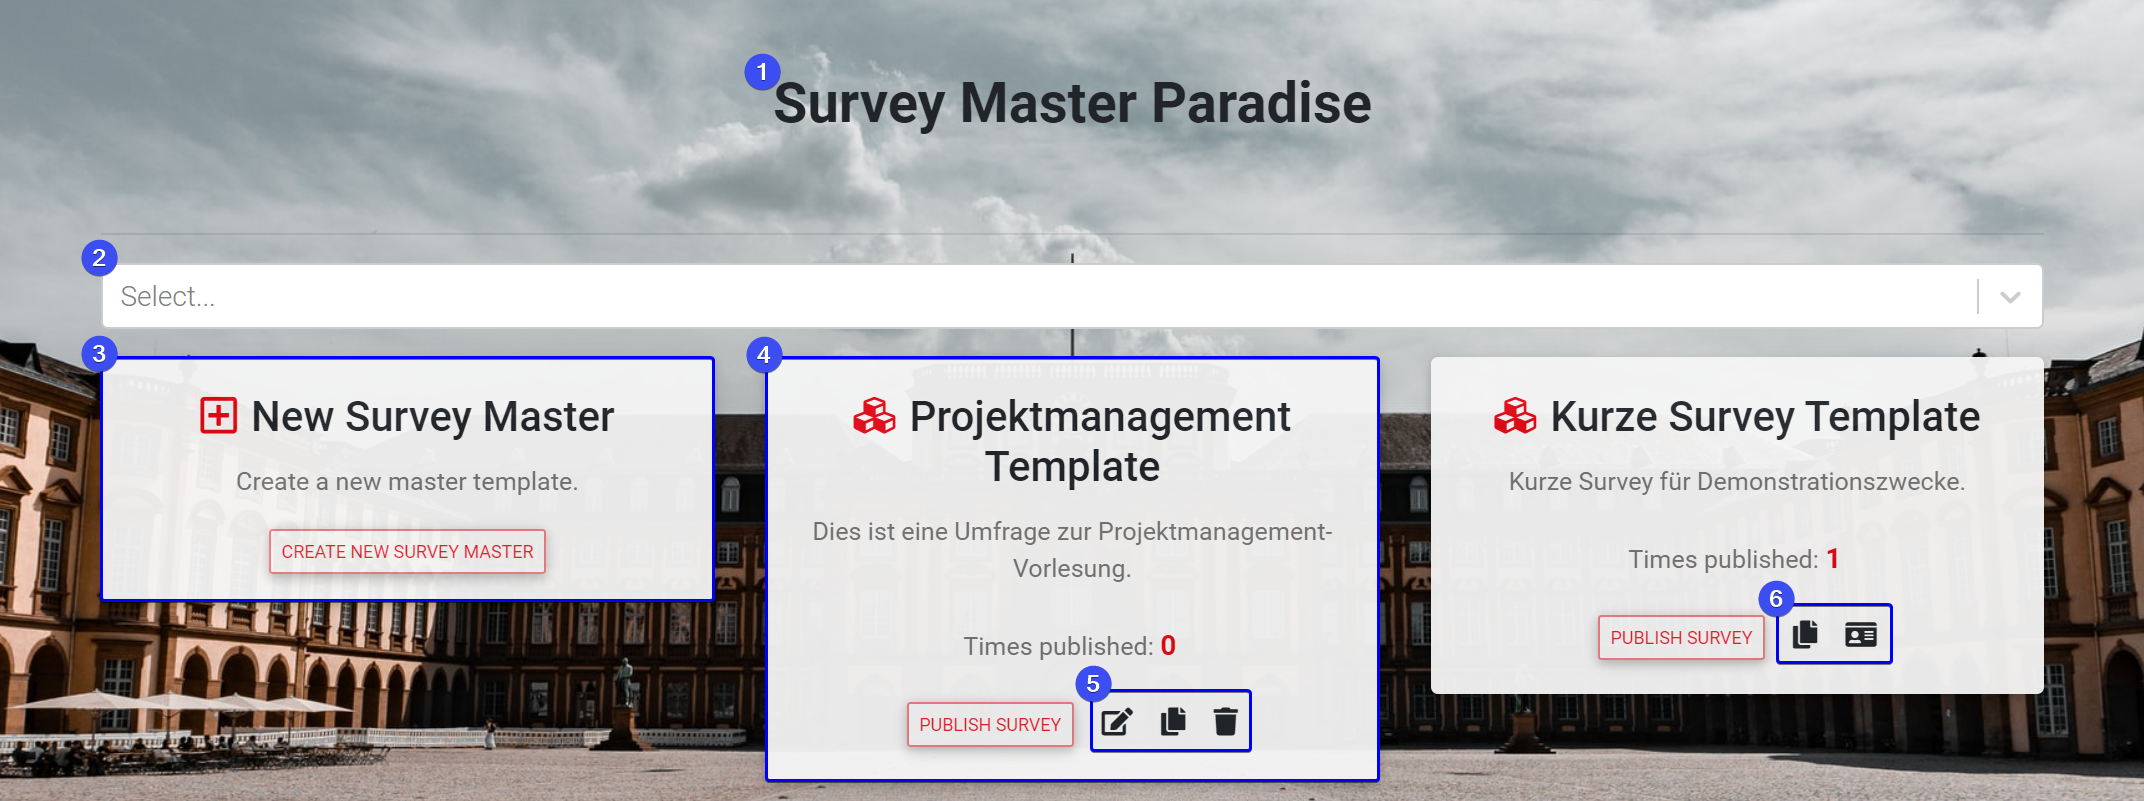
\includegraphics[width=0.95\textwidth, keepaspectratio]{img/guide/SurveyMasterParadise.png}
	\captionsetup{justification=centering, format=plain}
	\caption[Survey Master Paradise]{Survey Master Paradise \\\quelleScreenshot}
	\label{fig:SurveyMasterParadise}
\end{figure}

%%%%%%%%% --------------------- %%%%%%%%%%%%%%%
\subsection{Navigationsbereich}
\label{ssec:NavBar}

Die \abb \vref{fig:NavBar} stellt den für die angemeldeten Benutzer wie \zb den Dozenten \duzi oder die Studentin \ariane zur Verfügung stehende Funktionen dar. 
Die Benutzer können wie in \desOne auf ihre Ergebnissumfragen navigieren (vgl. Kap. \vref{ssec:ResultDashboard}). 
Dies könnte \ua wichtig für \ariane sein, um die Umfrageergebnisse ihrer Bachelorarbeit zu validieren. 
Oder über den in \desTwo dargestelltn Link auf ihre Umfragevorlagen (vgl. Kap. \vref{ssec:SurveyMasterParadise}). 
Hier kann \zb \duzi eine weitere Vorlage für seinen neuen Kurs \emph{WWWI20-MAC} anlegen und publizieren. 
 
Ferner zeigt die Navigationsleiste den Status \emph{Admin} \desThree, im Falle, dass der Benutzer ein administrative Rolle hat. \newline
Über das Icon \faUser[regular]\xspace \desFour kann der Benutzer zu seinem Account navigieren (vgl. Kap. \vref{ssec:EigenerAccount}). \newline
Über \desFive, dem Logout-Icon \faSignOut*\xspace, kann sich \duzi oder die Studentin \ariane vom System abmelden. 

\begin{figure}[H]
	\centering
	
\includegraphics[width=0.75\textwidth, keepaspectratio]{img/guide/NavBar.png}
	\captionsetup{justification=centering, format=plain}
	\caption[Navigationsbereich]{Navigationsbereich \\\quelleScreenshot}
	\label{fig:NavBar}
\end{figure}

%%%%%%%%% --------------------- %%%%%%%%%%%%%%%
\subsection{Meldungen}
\label{ssec:Meldungen}

Nachfolgend sind alle Meldungsarten mit Beispielen dargestellt.
Zunächst wird in \myRefGeneral{fig:approve} eine kurzzeitig eingeblendete Bestätigung dargestellt, welche eine Nachricht, die an den aktuellen Kontext angepasst ist beinhaltet.
Bestätigungen werden in den meisten Fällen automatisch ein- und ausgeblendet, um den Benutzerfluss nicht zu durchbrechen.
Im Beispiel wird dem Administrator bestätigt, dass er einen weiteren Nutzer zu einem neuen Administrator ernannt hat.

Auch abgelehnte oder abgebrochene Auftrage werden mit einer Nachricht versehen.
Diese beinhalten jedoch immer ein Knopf zur Bestätigung, sodass Fehlermeldungen auch notiert oder weiteren Personen gezeigt werden können.
Im Beispiel \myRefGeneral{fig:deny} wurde der Passwortänderungsauftrag des Nutzers \emph{Jansky} abgebrochen.

Auch Warnungen erhaltene eine besondere Darstellung.
Hierbei werden Änderungen, die eine Nutzereingabe benötigen, oder generelle Infos, die weder als negative noch als positive Benachrichtigung zählen, dargestellt.
Dazu wird in der Regel ebenfalls eine Bestätigung durch ein \emph{OK} oder eine explizite Auswahl, repräsentiert durch zwei Knöpfe, welche Kontextsensitiv sind, zur Bestätigung verwendet.
Im Beispiel \myRefGeneral{fig:warn} wird eine Umfrage veröffentlicht, welche einen eigenen Titel benötigt und somit ein Eingabefeld beinhaltet.

Zu guter Letzt gibt es weitere Sonderbenachrichtigungen, die wiederum kontextabhängig sind.
So ist etwa \abb \myRefGeneral{fig:special} die Bestätigung einer veröffentlichten Umfrage, welche nicht automatisch ausgeblendet wird, sondern aufgrund des besonderen Inhalts länger dargestellt wird und vom Nutzer selbst ausgeblendet werden muss.
Hierbei werden ebenfalls besondere Bestandteile visuell hervorgehoben, wie etwa der Surveycode in der Beispiel-Abbildung.

\begin{figure}[H]
	\centering
	
\includegraphics[width=0.5\textwidth, keepaspectratio]{img/guide/Angenommen.png}
	\captionsetup{justification=centering, format=plain}
	\caption[Beispiel Bestätigung]{Beispiel Bestätigung \\\quelleScreenshot}
	\label{fig:approve}
\end{figure}

\begin{figure}[H]
	\centering
	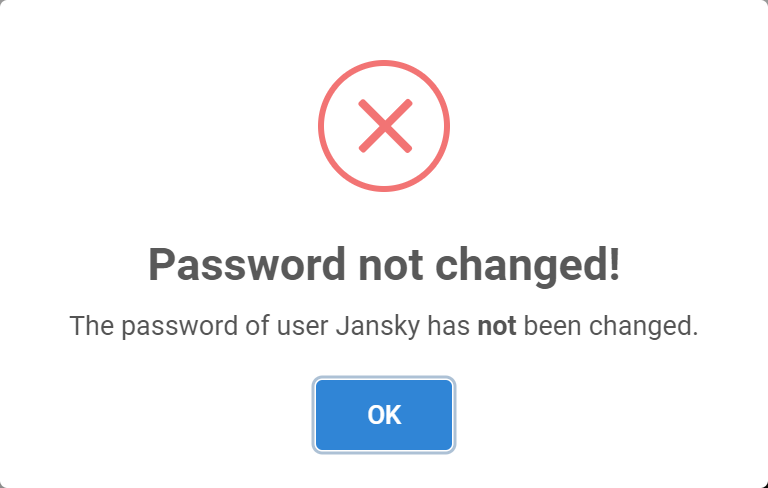
\includegraphics[width=0.5\textwidth, keepaspectratio]{img/guide/Abgelehnt.png}
	\captionsetup{justification=centering, format=plain}
	\caption[Beispiel Ablehnung]{Beispiel Ablehnung \\\quelleScreenshot}
	\label{fig:deny}
\end{figure}

\begin{figure}[H]
	\centering
	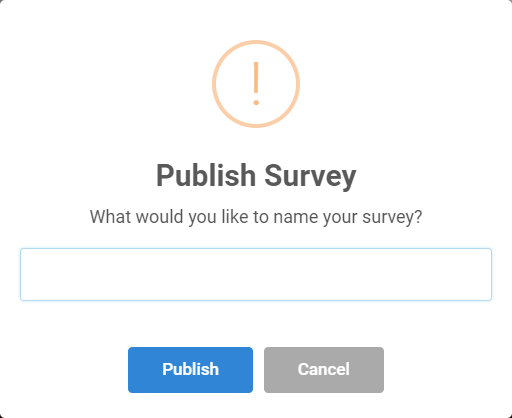
\includegraphics[width=0.5\textwidth, keepaspectratio]{img/guide/Publish.png}
	\captionsetup{justification=centering, format=plain}
	\caption[Beispiel Warnung mit Input]{Beispiel Warnung mit Input \\\quelleScreenshot}
	\label{fig:warn}
\end{figure}

\begin{figure}[H]
	\centering
	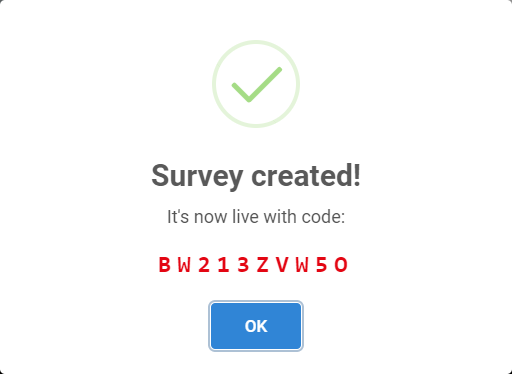
\includegraphics[width=0.5\textwidth, keepaspectratio]{img/guide/Published.png}
	\captionsetup{justification=centering, format=plain}
	\caption[Beispiel Bestätigung mit Zusatz]{Beispiel Bestätigung mit Zusatz \\\quelleScreenshot}
	\label{fig:special}
\end{figure}



